\section{Excavation in homogeneous media (3D)}
%\label{sec:e3d}
\subsubsection*{Problem definition}
A long round tunnel is build in the rock mass. The tunnel is 9 m lang and its radius is 0.33 m. We analyze the distribution of displacement and stresses after the excavtion. Different with the above section there is no plain stain at top the model. Fig. \ref{fme:e3d_g}

\begin{figure}[!htb]
  \begin{center}
    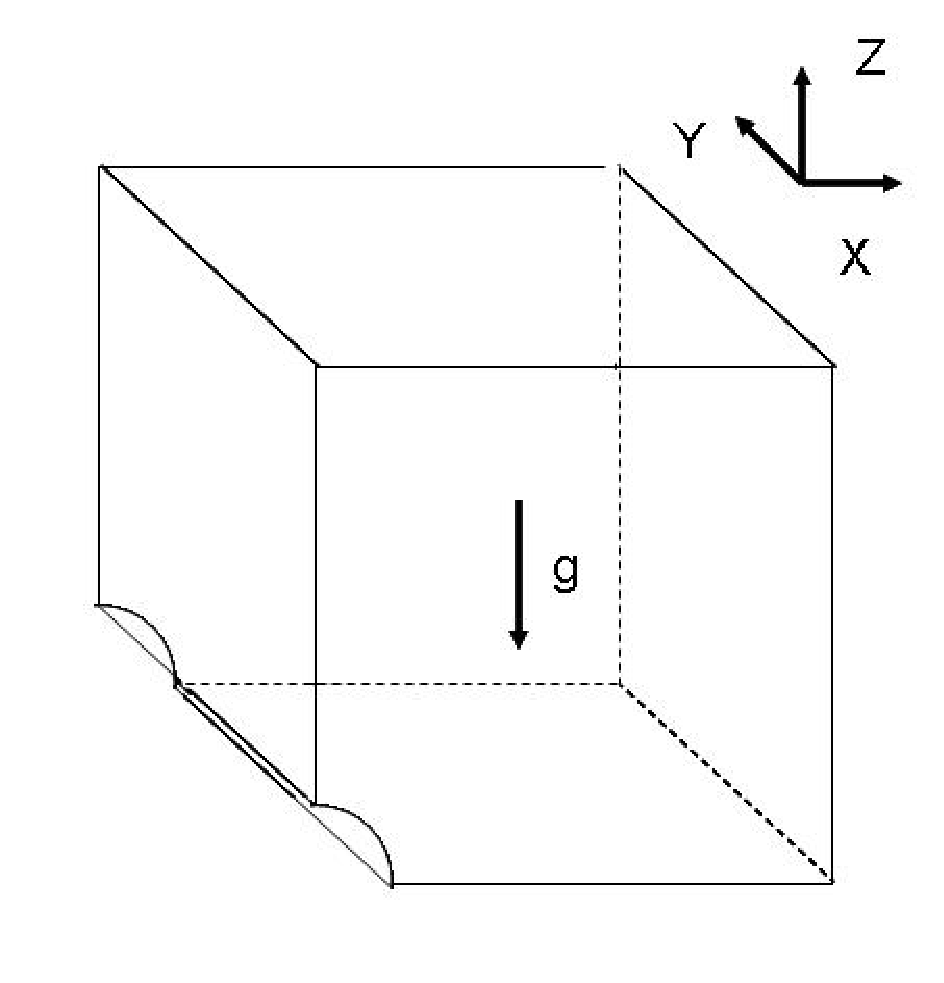
\includegraphics[scale=0.40]{M/e3d_g_model.eps}
  \end{center}
  \caption{Conceptual model of elastic foundation}
  \label{fme:e3d_g}
\end{figure}


\subsubsection*{Initial and boundary conditions}
The initial conditions are not required in this case. More detailed boundary conditions are illustrated in Fig. \ref{fme:e3d_g_bc}.
\begin{figure}[!hbt]
  \begin{center}
    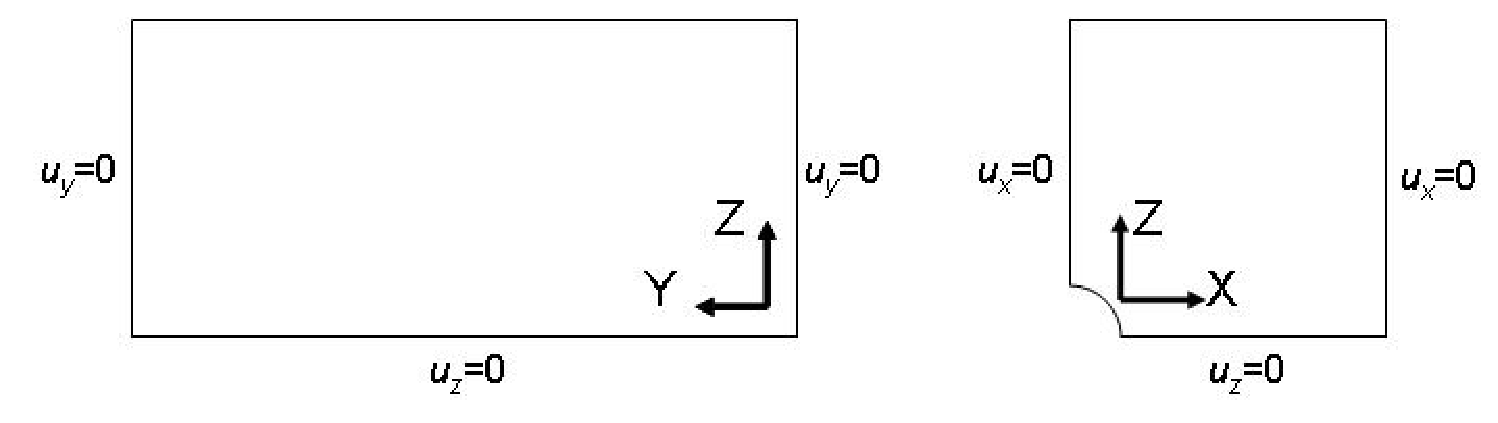
\includegraphics[scale=0.5]{M/e3d_g_bc.eps}
  \end{center}
  \caption{Boundary conditions}
  \label{fme:e3d_g_bc}
\end{figure} 
 

\subsubsection*{Material properties}

 \begin{table}[!htb]
\centering
\begin{tabular}{lll}
\hline\hline\noalign{\smallskip}
Property & Value & Unit \\
\noalign{\smallskip}\hline\noalign{\smallskip}
Young's modulus & $8$ & GPa \\
Poisson's ratio & $0.2$ & $-$ \\
Density & $2500$ & $kg/m^3$ \\
\noalign{\smallskip}\hline\hline
\end{tabular}
\caption{Parameters}
\label{tme:e3d_prop}
\end{table}

\subsubsection*{Results}
Fig. \ref{fme:e3d_disp} and \ref{fme:e3d_str} show the distribution of displacements and stresses after excavation. 

 \begin{figure}[!thb]
  \begin{center}
  \epsfig{figure=M/e3d_uz.eps,width=6cm, height=6cm}
  \epsfig{figure=M/e3d_ux.eps,width=6cm, height=6cm}
  \end{center}
  \caption{Distribution of displacement (m)}
  \label{fme:e3d_disp}
\end{figure}

\clearpage

 \begin{figure}[!thb]
  \begin{center}
  \epsfig{figure=M/e3d_szz.eps,width=6cm, height=6cm}
  \epsfig{figure=M/e3d_sxx.eps,width=6cm, height=6cm}
  \end{center}
  \caption{Distribution of stresses (Pa)}
  \label{fme:e3d_str}
\end{figure}

Fig. \ref{fme:e3d_diag} shows the radiral and tangential stresses in the X and Z direction. The results are compared to values obtained with FLAC3D version 3.10 and they are well mathed.

 \begin{figure}[!thb]
  \begin{center}
  \epsfig{figure=M/e3d_hori_diag.eps,width=6cm, height=6cm}
  \epsfig{figure=M/e3d_ver_diag.eps,width=6cm, height=6cm}
  \end{center}
  \caption{Distribution of stresses (Pa)}
  \label{fme:e3d_diag}
\end{figure} 

\subsubsection*{Benchmark deposit}

\begin{tabular}{|l|l|l|}
  \hline
  Benchmark & Problem type & Path in benchmark deposit \\
  \hline
 \emph{3d\_excav} & M & benchmarks\verb \M\excavation\3D_EX \\
  \hline
\end{tabular}